A Support Vector Machine(SVM) is a classifier which outputs an optimal hyperplane or set of hyperplanes in high-dimensional space and classifies new examples. In geometry, a Hyperplane in an n-dimensional space, is a subspace of one dimension less than the whole space. In figure \ref{fig:SVM} a hyperplane of 2-dimensional space is a line which divides the 2-dimensional space in half. This division defines two closed half-space. In other words, SVM is a supervised learning model that employs learning algorithms to recognize patterns and analyze data, used for classification of unknown data\cite{wiki:SVM}.\\
In figure \ref{fig:SVM} main idea behind SVM is shown. Consider example dataset described by variables $x_1$ and $x_2$ and suppose we want to classify all the elements(elements are shown by class circle and class square). The operation of SVM algorithm is based on finding the optimal hyperplane between training examples\cite{opencv_library}. An optimal hyperplane is one that gives the largest minimum distance to the training examples and it maximizes the margin between the hyperplane and all data points i.e. the best line that leaves the maximum margin from both classes.

\begin{figure}[H]
    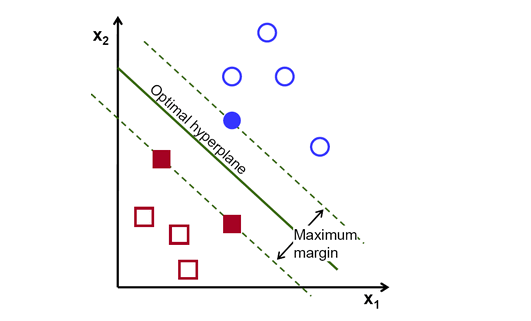
\includegraphics[width=0.45\textwidth]{./img/SVM.png}
     \caption{SVM for separable binary set}
    \label{fig:SVM}
\end{figure}

SVM are popular for couple of theoretical reasons: SVMs are robust to very large number of variables and can learn both simple and complex classification models\cite{cristianini2000}.\\

SVMs is a best known member in the general category of kernel methods\cite{shawe2004kernel}. A kernel method has the ability to generate non-linear decision boundaries by using method designed for linear classifiers. It turns out SVM does not need to work on higher-dimensional space implicitly because a kernel method rely on data through dot-products. Dot product can be replaced by kernel function which compute dot product in higher dimensional space. This allows the user to apply a classifier to data that has infinite- dimensional vector space representation such as DNA or protein\cite{ben2010user}.\\

In recent years, SVMs are widely used in bio-informatics \cite{furey2000support,osuna1997training,guyon2002gene} and other disciplines due to its ability to accurately deal with high dimensional data\cite{joachims1998text}. In marine environments , researches has proposed a method for detection of oil spills, from SAR data based on SVM classifier .The result of this research has shown that SVM has better performance on SAR image when using texture analysis and decomposition algorithm in various steps of the SVM algorithm. texture analysis will help to reduce noise in SAR image(SAR images are inherently noisy)\cite{matkan2013oil}.

 


